\documentclass[tikz,border=0cm]{standalone}
\usepackage{graphicx}
\usepackage{tikz}
\usetikzlibrary{positioning}
\usetikzlibrary{arrows,snakes,shapes,fadings,calc}
\usepackage{fontspec}
\setmainfont{Roboto}[
  Extension = .otf,
  UprightFont = *-Regular,
  BoldFont = *-Bold,
  ItalicFont = *-Italic,
  BoldItalicFont = *-BoldItalic,
]    
\usepackage{etoolbox} 

\newcommand{\figwidth}{7cm} 
\newcommand{\figheight}{10cm} 
\newcommand{\fontselect}{\large\bf} 


\begin{document}
\begin{tikzpicture}
 
  % Include the image in a node
  \node [
      above right,
      inner sep=0] (image) at (0,0) {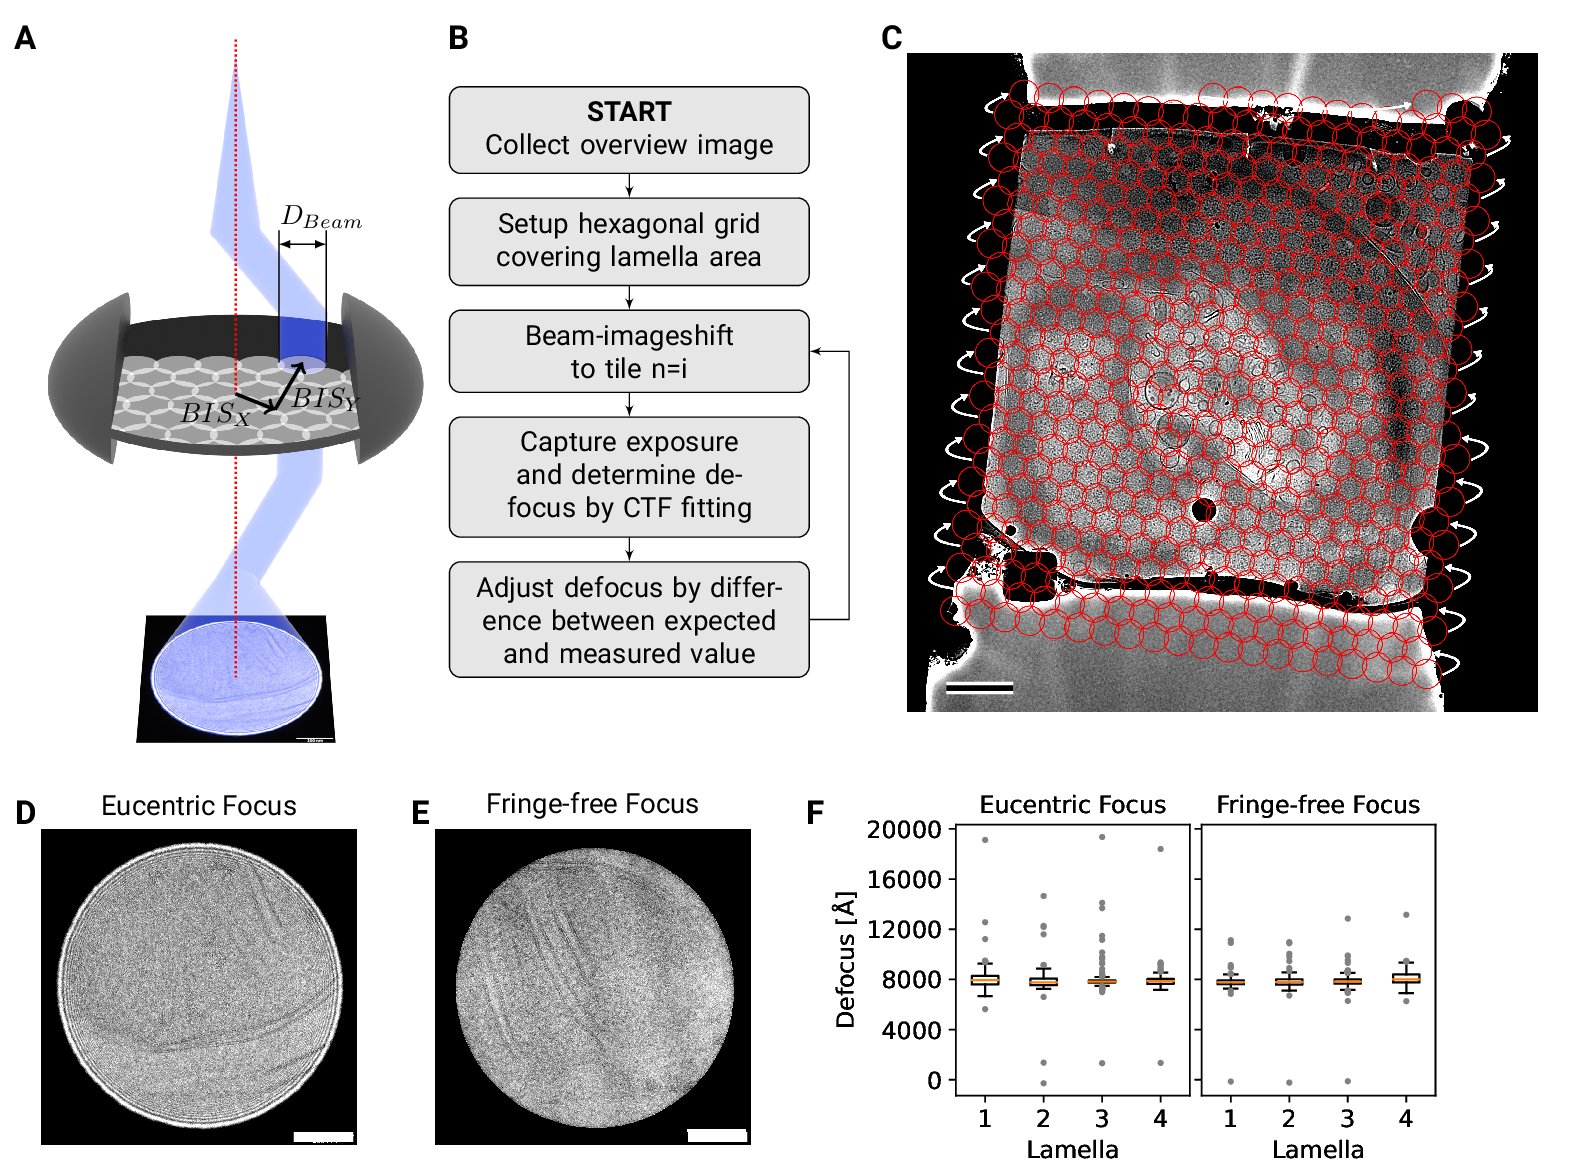
\includegraphics[width=\textwidth]{approach}};
   
  % Create scope with normalized axes
  \begin{scope}[
  x={($0.1*(image.south east)$)},
  y={($0.1*(image.north west)$)}]
   
  % Grid
      \draw[lightgray,step=1] (image.south west) grid (image.north east);
  \end{scope}
   
  \end{tikzpicture}
\end{document}